\chapter{Results and Discussion}
\label{ch:results}

\section{Purpose of This Chapter}

This chapter converts the progress-report material into a final-report results structure.
It already incorporates the synthetic findings currently available in the repository and leaves
a clear insertion point for the remaining real-route evaluation in Experiment~6.
That makes the document immediately usable as a strong final-report base while preserving a
clean path for the last empirical update.

\section{Current Synthetic Evaluation Snapshot}
\label{sec:current_synth_snapshot}

The repository currently contains processed synthetic results for Experiments~1, 2, 3, 4, 5,
and~7 under a reduced but reproducible benchmark profile.
These runs use 10 timed iterations per configuration, 0 warm-up iterations, base graph size
100 nodes, scalability sizes 100 and 1000 nodes, degree 5 unless otherwise varied, tank
capacity 40\,L unless otherwise varied, initial fuel 28\,L unless otherwise varied, and fuel
efficiency 10\,km/L.
The resulting dataset contains 1,460 timed runs and is sufficient to support a substantive
comparative discussion of the implemented algorithms.

\begin{table}[H]
    \centering
    \caption{Current synthetic execution profile used to populate the final-report scaffold.}
    \label{tab:final_current_synth_profile}
    \begin{tabular}{ll}
        \toprule
        Setting & Value \\
        \midrule
        Timed runs per configuration & 10 \\
        Warm-up runs per configuration & 0 \\
        Base graph size & 100 nodes \\
        Scalability graph sizes & 100, 1000 nodes \\
        Approximate degree & 5 \\
        Default tank capacity & 40\,L \\
        Default initial fuel & 28\,L \\
        Fuel efficiency & 10\,km/L \\
        Total result rows & 1,460 \\
        Covered experiments & 1, 2, 3, 4, 5, and 7 \\
        \bottomrule
    \end{tabular}
\end{table}

\section{Cross-Experiment Findings}

\subsection*{Experiment 1: Scalability}

The currently available scalability results already separate PF-A* from the other methods in
practical terms.
At 1000 nodes, PF-A* matches the best mean cost of 2876.88 while reducing mean runtime to
552.37\,ms, compared with 1771.17\,ms for State-Expanded Dijkstra and 1640.96\,ms for
Dynamic Programming.
Standard A* and RF-A* are both much slower at this scale in the present implementation,
while the Greedy baseline is infeasible on the tested instances.

\begin{figure}[H]
      \centering
      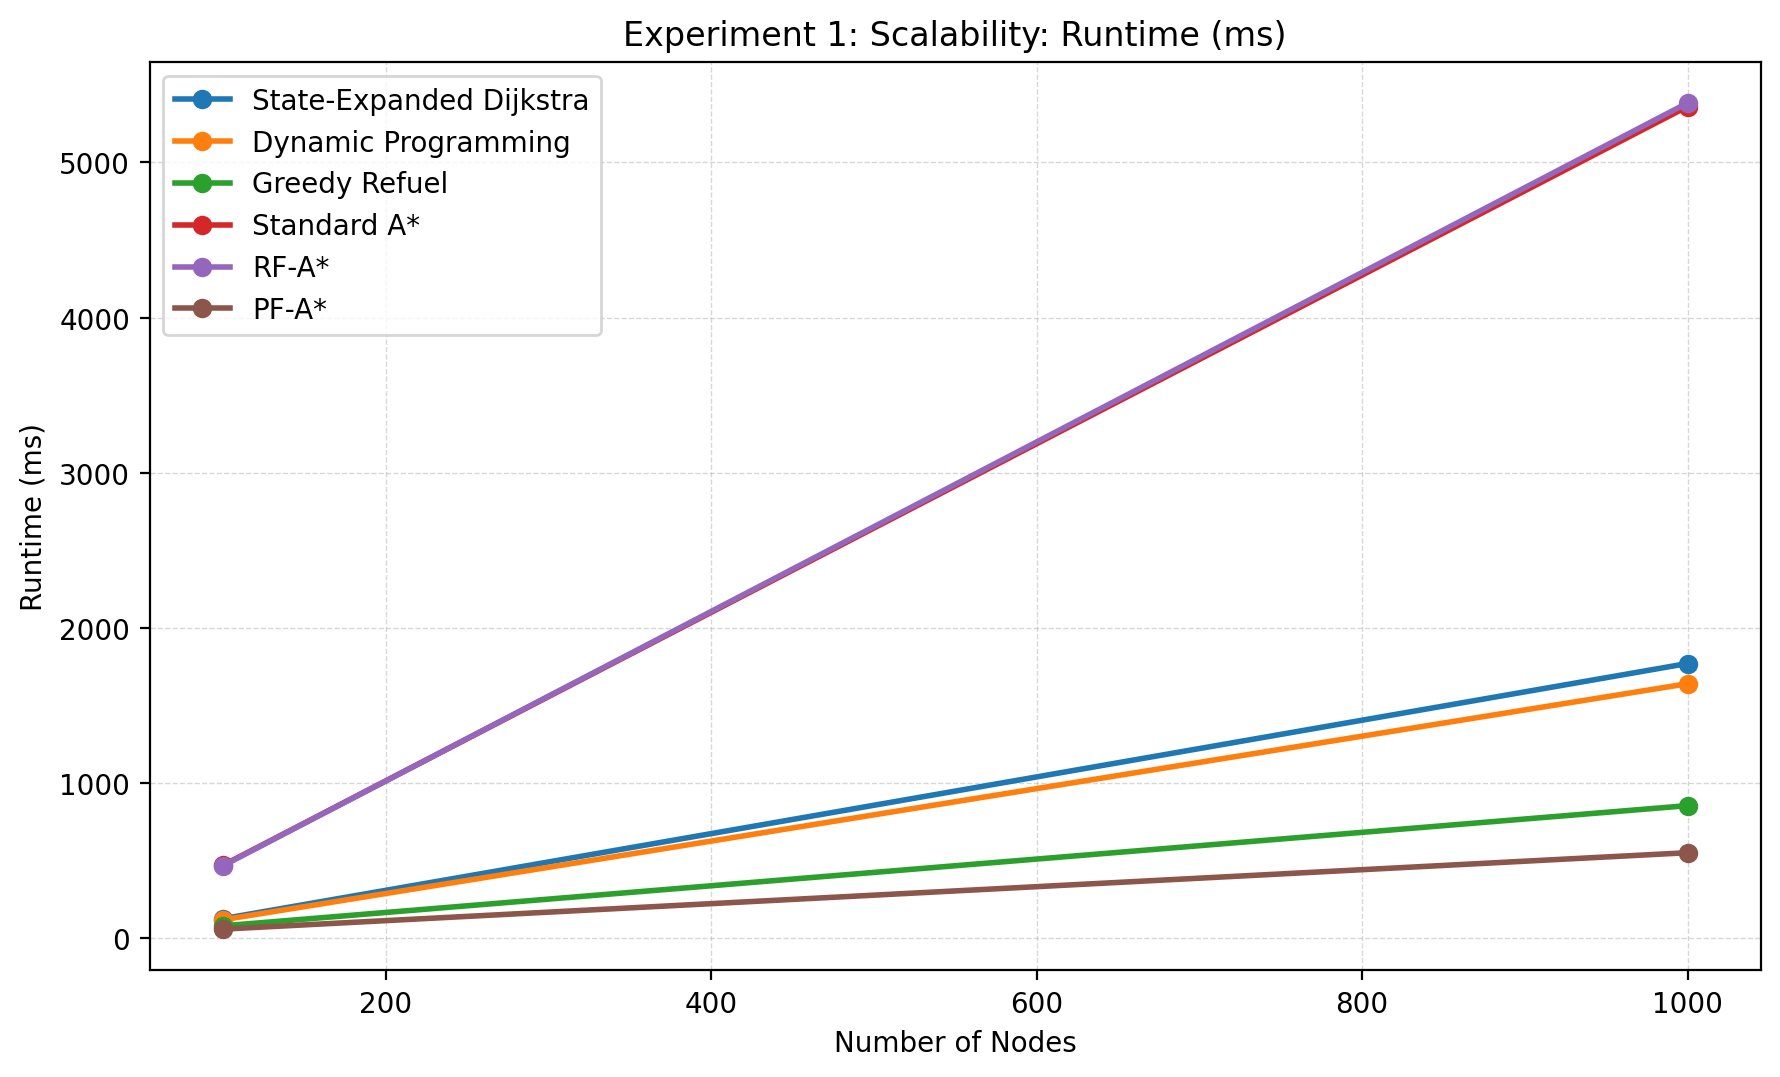
\includegraphics[width=0.90\textwidth]{../results/report_assets/exp1_scalability/exp1_scalability_runtime.png}
      \caption{Experiment~1 runtime as graph size increases. PF-A* remains much faster than the exact baselines in the current synthetic profile while matching their best observed mean cost.}
      \label{fig:final_exp1_runtime}
\end{figure}

\subsection*{Experiment 2: Fuel Price Variance}

Increasing price variance strengthens the value of cost-aware purchase decisions.
The best observed mean cost falls from 3528.00 at $\sigma=0\%$ to 2576.21 at $\sigma=20\%$,
and PF-A* stays on that best-cost curve throughout the tested range.
This behaviour matches the theoretical intuition of the problem: selective refuelling becomes
more valuable as the spread between cheap and expensive stations widens.

\begin{figure}[H]
      \centering
      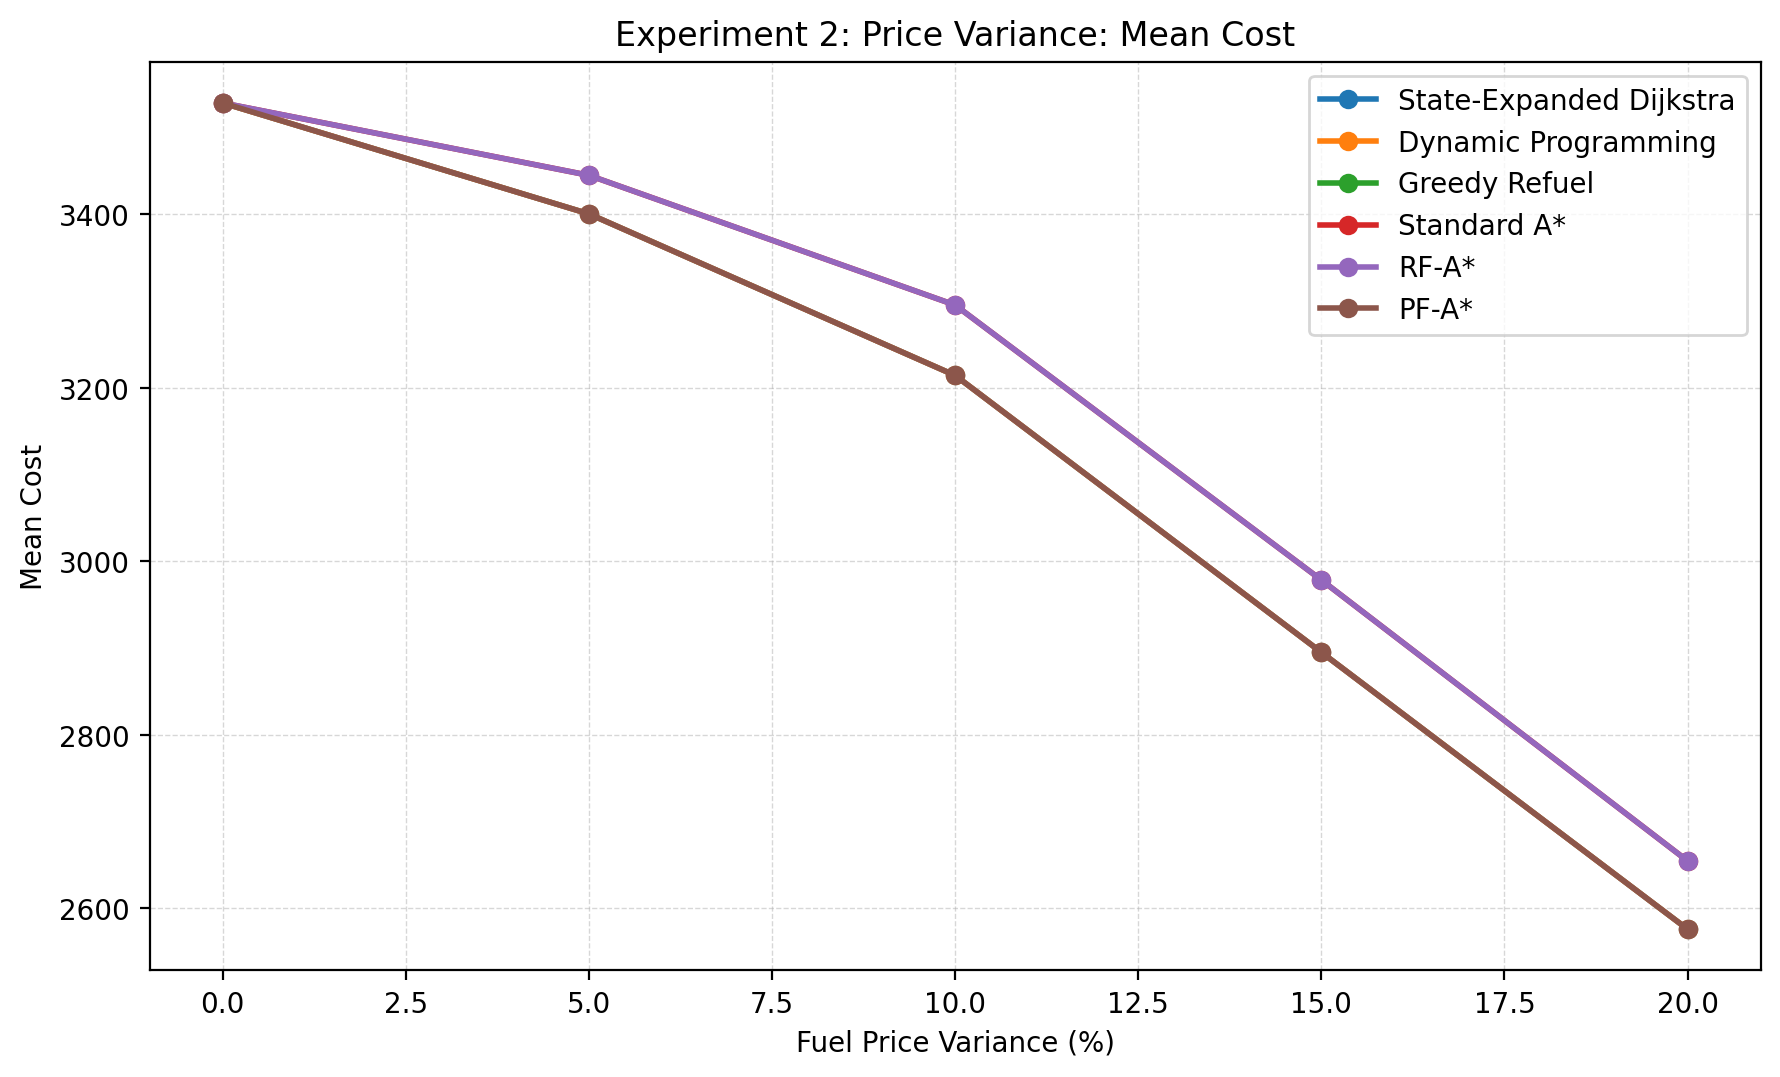
\includegraphics[width=0.90\textwidth]{../results/report_assets/exp2_price_variance/exp2_price_variance_cost.png}
      \caption{Experiment~2 mean cost under increasing fuel-price variance. Larger variance creates more opportunity to save money through selective purchasing.}
      \label{fig:final_exp2_cost}
\end{figure}

\subsection*{Experiment 3: Tank Capacity}

Larger tanks reduce fuel cost but enlarge the effective state space.
Across the tested configurations, the best observed mean cost drops from 3922.82 at 20\,L to
2185.84 at 80\,L, while the runtime of the exact methods grows sharply.
PF-A* preserves the same best observed cost curve while keeping the runtime increase much
smaller than that of the exact state-expanded baselines.

\begin{figure}[H]
      \centering
      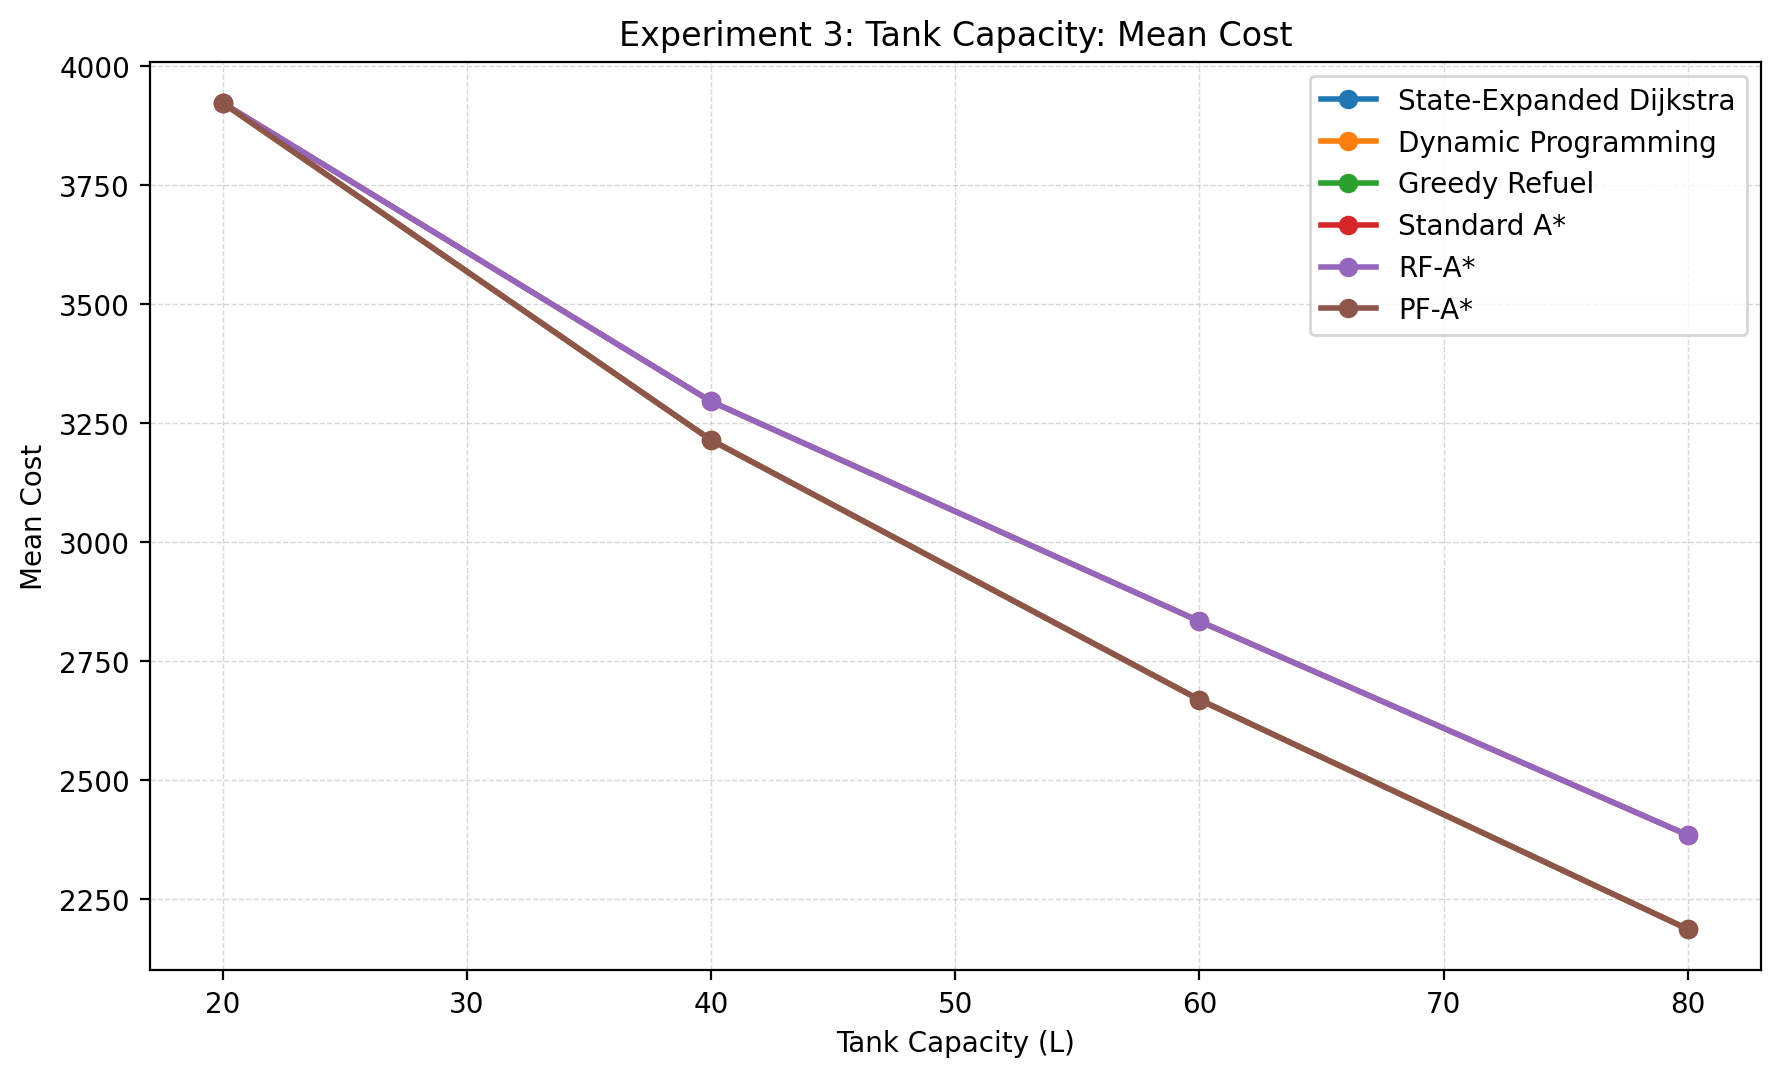
\includegraphics[width=0.90\textwidth]{../results/report_assets/exp3_tank_capacity/exp3_tank_capacity_cost.png}
      \caption{Experiment~3 mean cost as tank capacity varies. Larger tanks create more opportunities to defer purchasing to cheaper stations, but they also increase computational burden.}
      \label{fig:final_exp3_cost}
\end{figure}

\subsection*{Experiment 4: Initial Fuel}

Higher initial fuel reduces both cost and search effort.
For the optimal methods in the current dataset, mean cost decreases from 3848.58 at 10\,L
initial fuel to 2831.54 at 40\,L, and PF-A* also becomes faster as the initial fuel level
increases.
This is consistent with the fact that higher starting fuel weakens the urgency of early
refueling decisions.

\begin{figure}[H]
      \centering
      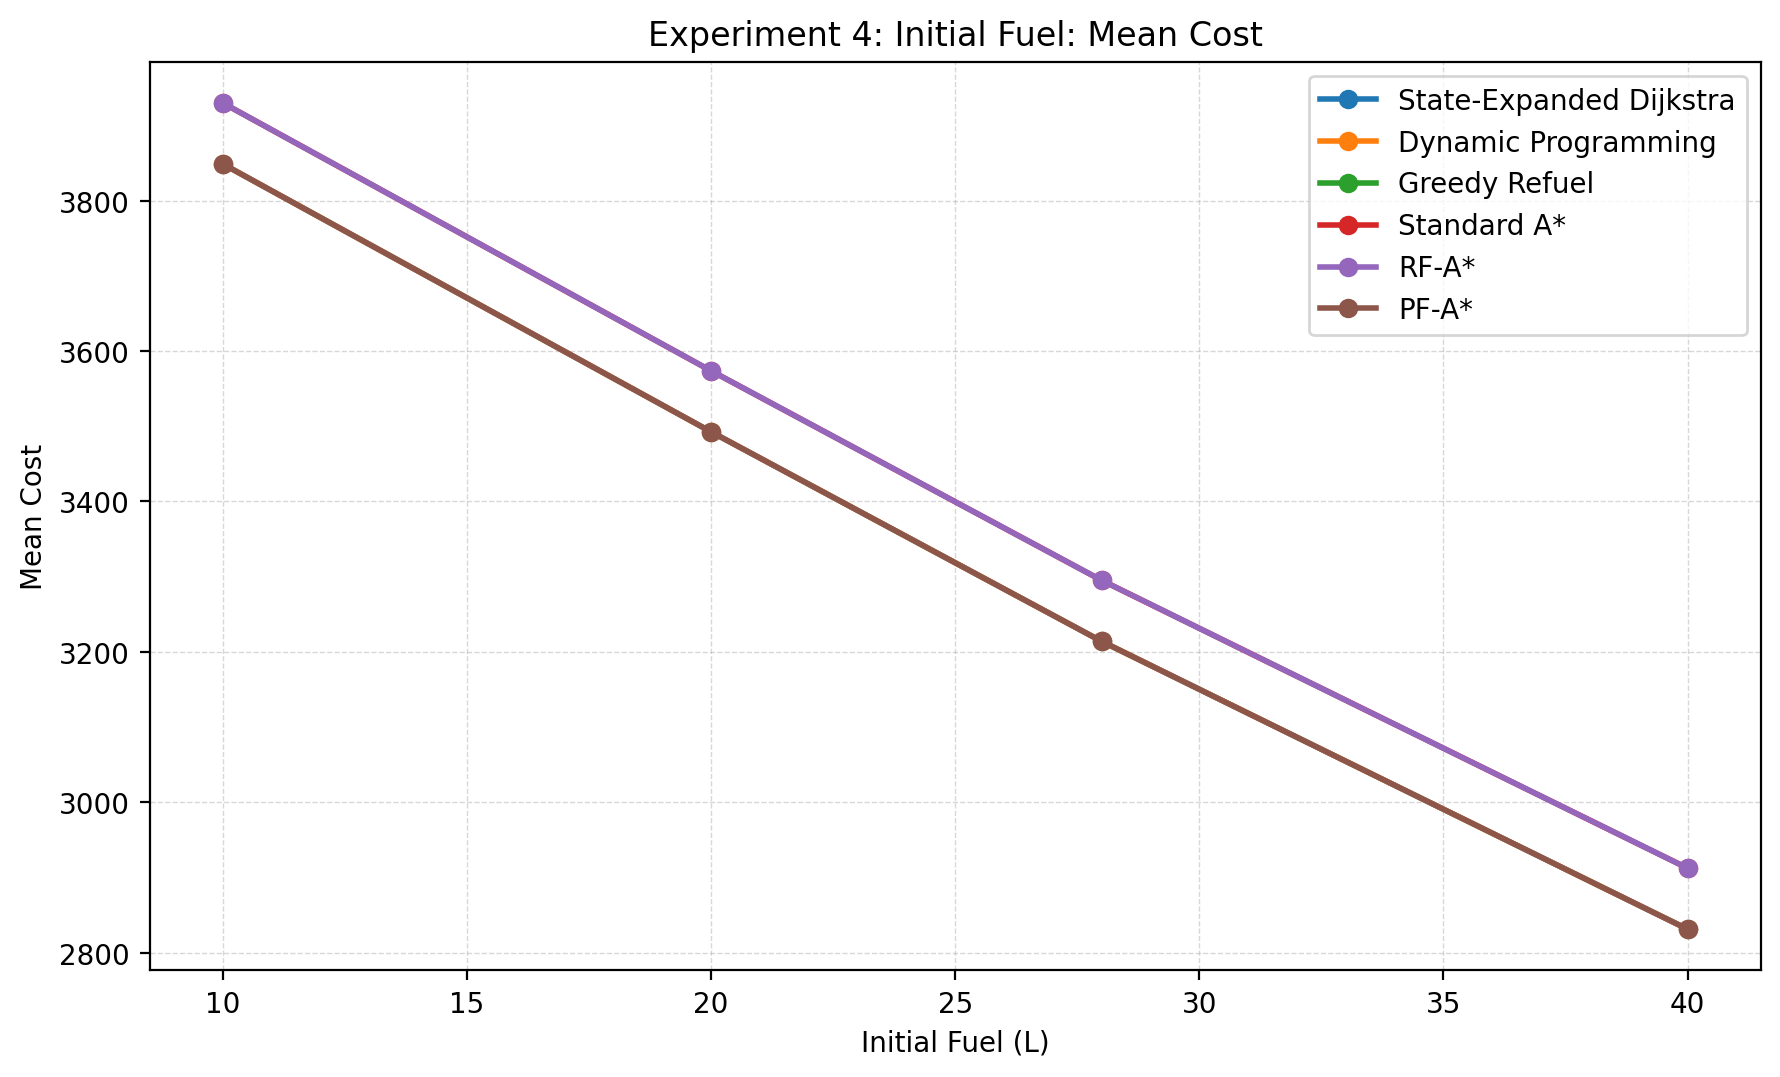
\includegraphics[width=0.90\textwidth]{../results/report_assets/exp4_initial_fuel/exp4_initial_fuel_cost.png}
      \caption{Experiment~4 mean cost as initial fuel varies. Starting with more fuel lowers the need for costly early purchases.}
      \label{fig:final_exp4_cost}
\end{figure}

\subsection*{Experiment 5: PF-A* versus RF-A*}

Experiment~5 remains the central novelty experiment for the proposed heuristic.
Across the feasible tested configurations, PF-A* is substantially faster than RF-A* and expands
far fewer states.
At degree 5 and $\sigma=10\%$, PF-A* requires 2115 expanded states and 59.92\,ms on average,
while RF-A* requires 18,507 expanded states and 475.48\,ms.

At the same time, the present dataset reveals an implementation issue that must be discussed
explicitly: Standard A* and RF-A* do not currently match the best observed costs returned by
State-Expanded Dijkstra, Dynamic Programming, and PF-A*.
That mismatch should be treated as a correctness or implementation-audit item rather than
hidden as noise.
For a final submitted dissertation, the strict-profile rerun should only be performed after
this discrepancy is resolved.

\begin{table}[H]
    \centering
    \caption{Representative Experiment~5 comparison at $\sigma=10\%$.}
    \label{tab:final_exp5_sigma10}
    \begin{tabular}{lcccc}
        \toprule
        Algorithm & Degree & Feasible (\%) & Mean Cost & Mean Runtime (ms) \\
        \midrule
        RF-A* & 5  & 100 & 3295.18 & 475.48 \\
        PF-A* & 5  & 100 & 3214.11 & 59.92 \\
        RF-A* & 10 & 100 & 2944.98 & 518.06 \\
        PF-A* & 10 & 100 & 2794.91 & 80.49 \\
        RF-A* & 20 & 100 & 2752.33 & 422.48 \\
        PF-A* & 20 & 100 & 2554.99 & 82.57 \\
        \bottomrule
    \end{tabular}
\end{table}

\begin{figure}[H]
      \centering
      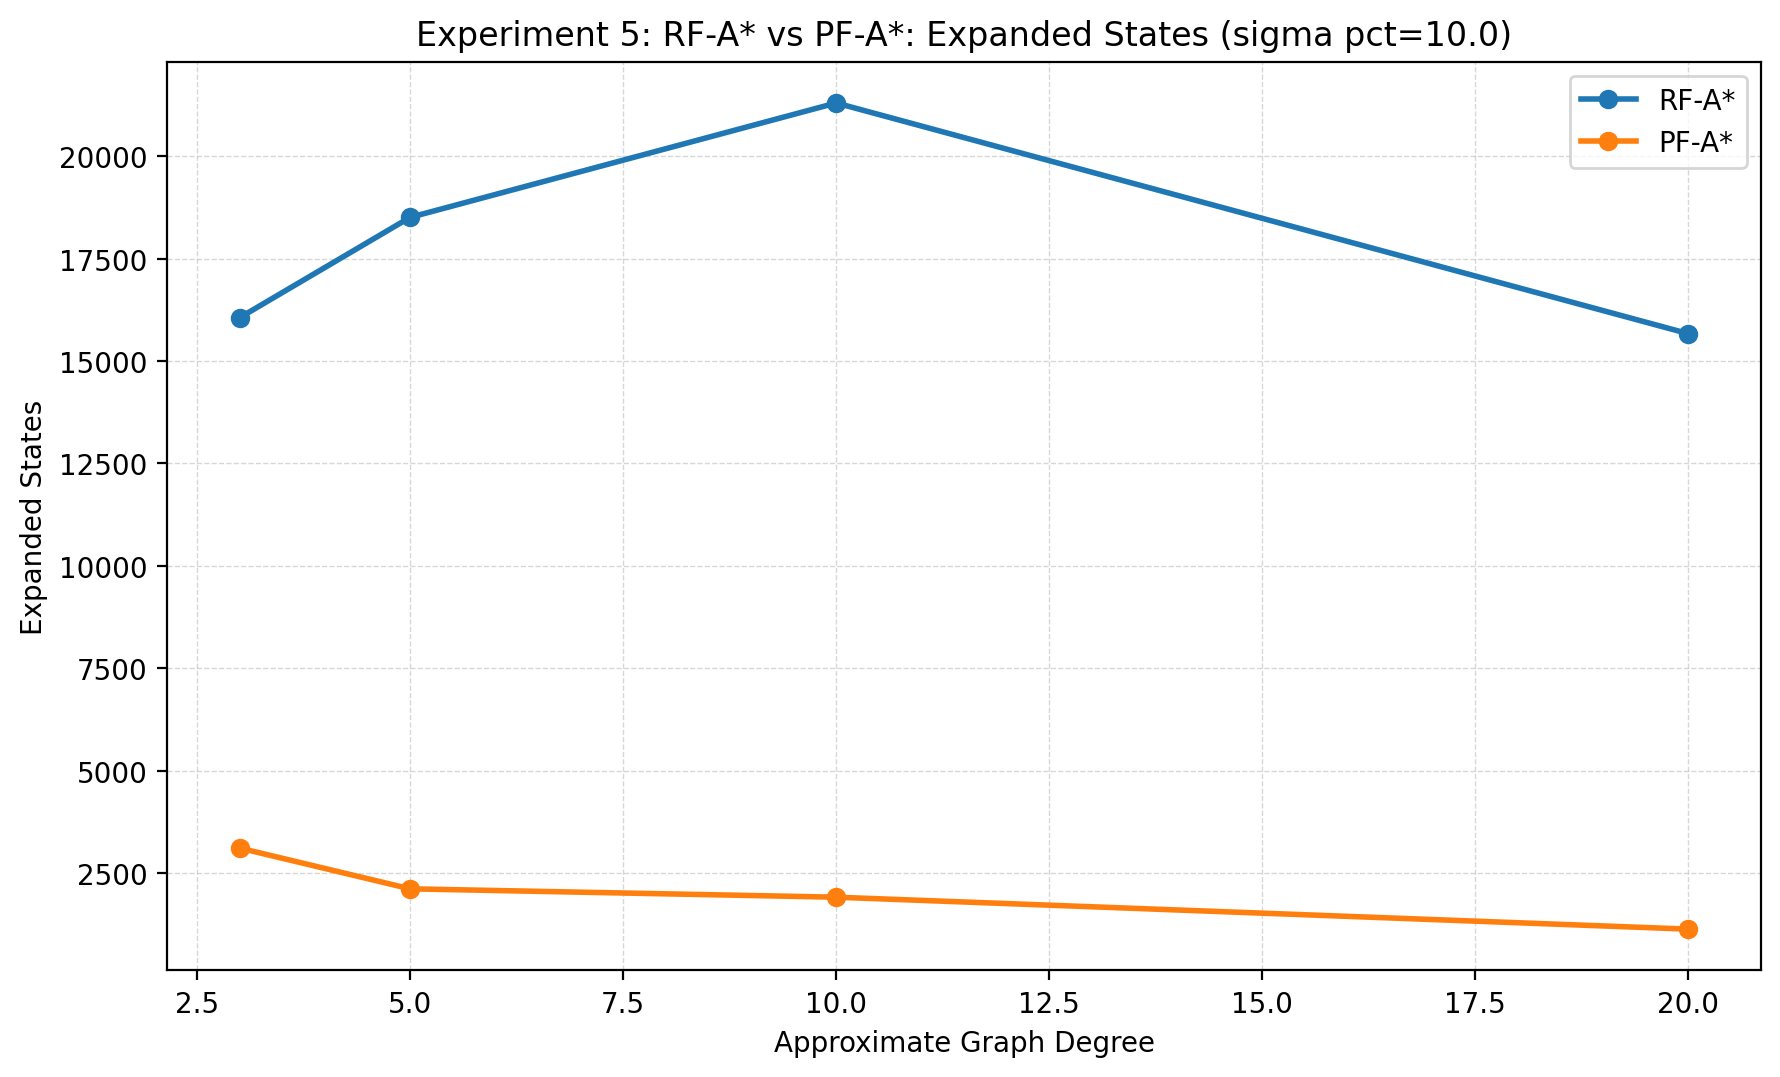
\includegraphics[width=0.90\textwidth]{../results/report_assets/exp5_rf_vs_pf/exp5_rf_vs_pf_expanded_states_sigma_pct_10_0.png}
      \caption{Experiment~5 node expansions for RF-A* and PF-A* at $\sigma=10\%$. PF-A* explores substantially fewer states in the tested feasible density regimes.}
      \label{fig:final_exp5_expanded}
\end{figure}

\subsection*{Experiment 7: Variable Purchase versus Full-Tank-Only}

Experiment~7 shows that the variable-purchase model delivers meaningful economic value.
Across the 16 tested $(\sigma, C)$ combinations, the full-tank-only baseline incurs an average
cost penalty of 10.86\%, with observed penalties ranging from 1.19\% to 24.81\%.
The computational overhead of the variable-purchase model is real, but so are the monetary
savings it enables.

\begin{table}[H]
    \centering
    \caption{Representative Experiment~7 comparison at $\sigma=10\%$.}
    \label{tab:final_exp7_sigma10}
    \begin{tabular}{lccc}
        \toprule
        Tank capacity (L) & Variable-purchase cost & Full-tank-only cost & Cost gap (\%) \\
        \midrule
        20 & 3922.82 & 4137.17 & 5.46 \\
        40 & 3214.11 & 3611.20 & 12.35 \\
        60 & 2668.14 & 2799.09 & 4.91 \\
        80 & 2185.84 & 2728.20 & 24.81 \\
        \bottomrule
    \end{tabular}
\end{table}

\begin{figure}[H]
      \centering
      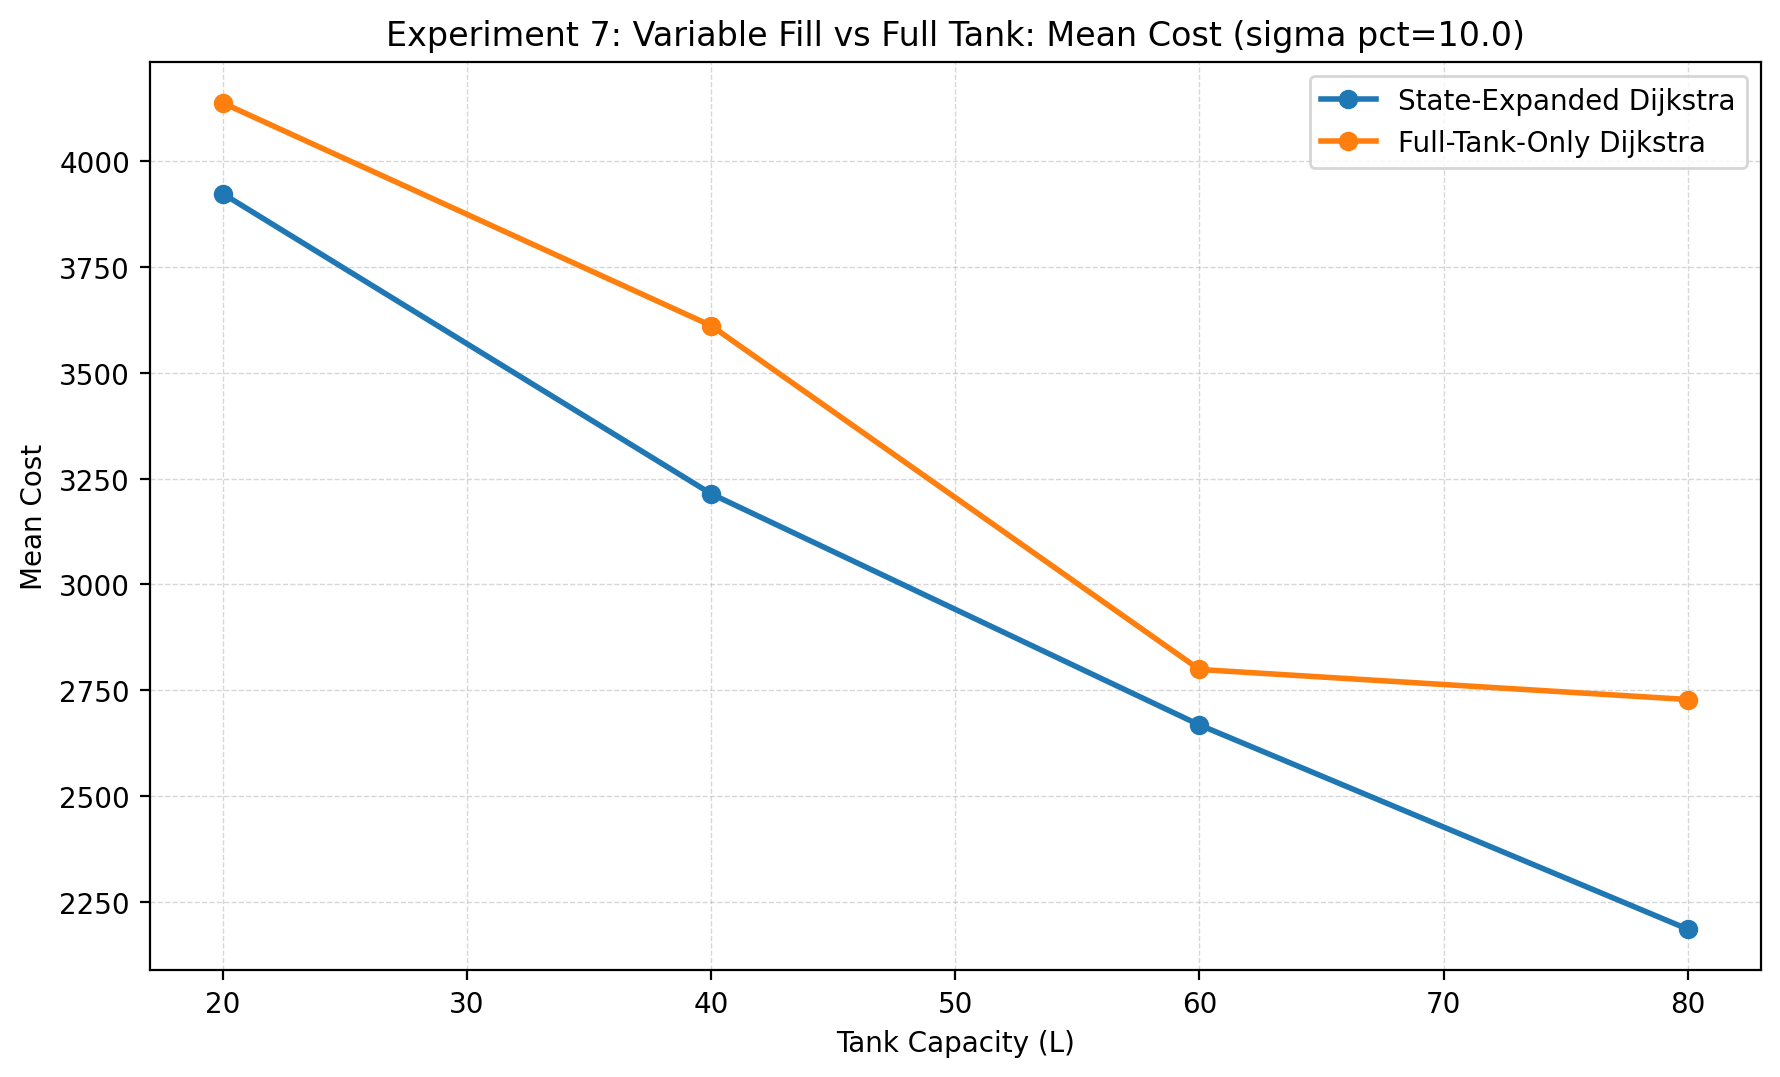
\includegraphics[width=0.90\textwidth]{../results/report_assets/exp7_variable_vs_full_tank/exp7_variable_vs_full_tank_cost_sigma_pct_10_0.png}
      \caption{Experiment~7 mean cost at $\sigma=10\%$ under the variable-purchase and full-tank-only models. Variable purchase remains cheaper across all tested tank capacities.}
      \label{fig:final_exp7_cost}
\end{figure}

\section{Integrated Interpretation}

Three conclusions are already well supported by the present repository results.
First, PF-A* is the strongest overall algorithm in the currently tested synthetic setting: it
matches the best observed cost where the exact methods agree, while reducing runtime and node
expansions substantially.
Second, modelling variable purchase decisions is empirically worthwhile, since the
full-tank-only baseline pays a repeated cost penalty across the tested configurations.
Third, the current evaluation pipeline is useful not only for showcasing strengths but also for
surfacing implementation defects, most notably the cost mismatch observed for Standard A* and
RF-A*.

\section{Experiment~6 Integration Section}
\label{sec:exp6_integration}

The remaining real-route evaluation should be inserted into this final report as a substantive
empirical section rather than a brief appendix.
The repository is already structured for that update.

\subsection*{Data and Execution Path}

The recommended data and execution flow is:
\begin{enumerate}
    \item Define the three corridors in \texttt{data/real\_routes/corridors.example.json} or a project-specific copy.
    \item Collect road-network and fuel-station data with \path{scripts/run_windows_collect_real_route_data.ps1}.
    \item Store cleaned route instances in \texttt{data/real\_routes/generated/<instance>.json}.
    \item Run Experiment~6 through \path{scripts/run_windows_real_experiments.ps1} or \path{scripts/run_real_experiments.py}.
    \item Summarize the resulting \texttt{real\_route\_results.csv} into report tables and figures.
\end{enumerate}

\subsection*{Recommended Final-Report Content for Experiment~6}

When the real-route results are ready, this chapter should be extended with:
\begin{itemize}
    \item a route-by-route table covering feasibility, cost, runtime, and expanded states,
    \item a comparison between variable purchase and full-tank-only costs for each corridor,
    \item one figure per corridor showing station prices or refuelling points along the route,
    \item a discussion of whether the synthetic trends transfer to the Thai road network, and
    \item a brief audit note confirming whether RF-A* and Standard A* were repaired before the final run.
\end{itemize}

\section{Limitations}

Two limitations should remain explicit in any final submission built from the current
repository snapshot.
First, the synthetic results embedded in this scaffold come from a reduced profile rather than
the full 10,000-run target.
Second, the observed discrepancy in Standard A* and RF-A* means that strict claims about all
optimal algorithms agreeing should not be made until the implementation audit is complete.
